\documentclass[xcolor=dvipsnames,10pt]{beamer}
% ********** Style prezentation **********

\usepackage{verbatim}
\usepackage{color}
\usepackage{multimedia}
\usepackage{xmpmulti}
\usepackage[absolute,overlay]{textpos} 
\usepackage{listings}
\usepackage{algorithm}
\usepackage{algorithmic}
\usepackage{amsmath}
\usepackage{pifont}
\usepackage{url}
\usepackage{pict2e}
\usepackage{flushend}
\usepackage{graphicx}
\usepackage{pgf}
\usepackage{url}
\usepackage{tikz}
\usetikzlibrary{calc}
\usetikzlibrary{shapes}
\usetikzlibrary{backgrounds}
\usepackage{pgfplots}
\usepackage{pgfplotstable}

\newcommand{\ignore}[1]{}


\lstset{ %
  language=Java,              
  basicstyle=\footnotesize
}

\mode<presentation>
{
	\usetheme{Warsaw}
}
\definecolor{scarlet}{RGB}{200,0,0}
\setbeamercolor{structure}{fg=scarlet}
\addtobeamertemplate{footline}{
\begin{columns}
  \hfill\includegraphics[height=.75cm]{unl_clear.pdf}\hspace{.5cm}
\end{columns}
\vspace{2mm}
}{\usebeamercolor[bg]{footline}\hfill\raisebox{1mm}[0mm]{\hspace{2mm}}}

\newcommand\x[1]{\ensuremath{\mathit{#1}}}
\newcommand\lrangle[1]{\ensuremath{\langle#1\rangle}}

\def\ON{\ding{52}}
\def\OF{\ding{55}}
\def~{\phantom{0}}

\setbeamertemplate{navigation symbols}{} %remove if navigation symbols are needed
\setbeamersize{text margin left=5mm, text margin right=5mm} % change margin as you wish

\author{Matthew B. Dwyer}

\title[Probabilistic Program Analysis]{Probabilistic Program Analysis}
\subtitle{Symbolic Execution + Model Counting + Reinforcement Learning}


\institute{
Department of Computer Science and Engineering\\
University of Nebraska - Lincoln\\
Lincoln, Nebraska USA\\
}

\date{Summer 2014}

\begin{document}

\begin{frame}
	\titlepage %displays the title page
\end{frame}

\begin{frame}{Program Correctness}
\vfill
How do you tell if your program works correctly?\\
{\center (hint: this is a two part answer)}
\vfill
\pause
\begin{itemize}
\item Specify what it means to be correct
\pause
\vfill
\item Provide evidence that the program's behavior matches the specification
\end{itemize}
\vfill
\end{frame}

\begin{frame}{Program Correctness}
\vfill
How can you specify what it means to be correct?
\pause
\begin{itemize}
\item oracle: $completeTriple(a,b)=c \iff 
\sqrt{a^2 + b^2} = c \vee
\sqrt{a^2 + c^2} = b \vee \ldots$
\pause
\item assert: \texttt{assert a > 0;}
\end{itemize}
\pause
\vfill
What kind of evidence can you provide?
\begin{itemize}
\item read the code\pause
\item testing: $completeTriple(3,4)=c \iff \sqrt{3^2 + 4^2} = \sqrt{25} = 5 = c \vee \ldots$
\pause
\end{itemize}
\vfill
Wouldn't it be nice if you could systematically check all/most of the program's behavior against the specification?
\vfill
\end{frame}

\begin{frame}[fragile]
\frametitle{Program analysis in a nutshell}
\vfill
Consider the following program fragment:
\vfill
\begin{minipage}[t]{0.4\textwidth}
\lstset{numbers=left, numbersep=2pt}
\begin{center}
\begin{lstlisting}
int classify(int a, int b, int c) {
  if (a==b) 
    type+=1;
  if (a==c) 
    type+=2;
  if (b==c) 
    type+=3;
  assert type != 6; ...
\end{lstlisting}
\end{center}
\end{minipage}
\hfill
\uncover<2>{
\begin{minipage}[t]{0.4\textwidth}
A \textbf{set} of program traces
\begin{align*}
\{ & [1,2,4,6,8],\\
   & [1,2,3,4,6,8],\\
   & [1,2,4,5,6,8],\\
   & [1,2,4,6,7,8],\\
   & \ldots \}
\end{align*}
\end{minipage}
}
\vfill
Is there a trace that leads to the \texttt{assert} being violated?
\end{frame}

\begin{frame}[fragile]
\frametitle{Program analysis in a nutshell}
\vfill
Consider the following program fragment:
\vfill

\begin{minipage}[t]{0.4\textwidth}
\lstset{numbers=left, numbersep=2pt}
\begin{center}
\begin{lstlisting}
int classify(int a, int b, int c) {
  if (a==b) 
    type+=1;
  if (a==c) 
    type+=2;
  if (b==c) 
    type+=3;
  assert type != 6; ...
\end{lstlisting}
\end{center}
\end{minipage}
\hfill
\begin{minipage}[t]{0.4\textwidth}
A \textbf{tree} of program traces
\begin{tikzpicture}[scale=0.6, sibling distance=20pt, level distance=30pt]
 \node {1}
  child {
   node {2}
    child {
     node[xshift=-7mm] {3}
      child {
       node {4}
        child {
         node[xshift=-3mm] {5}
          child {
           node {6}
            child {
             node {7}
              child {
               node {8}
               edge from parent
              }
             edge from parent
            }
            %child {
            % node {8}
            % edge from parent
            %}
           edge from parent
          }
         edge from parent
        }
        child {
         node[xshift=3mm] {6}
          %child {
          % node {7}
          %  child {
          %   node {8}
          %   edge from parent
          %  }
          % edge from parent
          %}
          child {
           node {8}
           edge from parent
          }
         edge from parent
        }
       edge from parent
      }
     edge from parent
    }
    child {
     node[xshift=7mm] {4}
        child {
         node[xshift=-3mm] {5}
          child {
           node {6}
            %child {
            % node {7}
            %  child {
            %   node {8}
            %   edge from parent
            %  }
            % edge from parent
            %}
            child {
             node {8}
             edge from parent
            }
           edge from parent
          }
         edge from parent
        }
        child {
         node[xshift=3mm] {6}
          child {
           node {7}
            child {
             node {8}
             edge from parent
            }
           edge from parent
          }
          child {
           node {8}
           edge from parent
          }
         edge from parent
     edge from parent
    }
   edge from parent
  }
 };
\end{tikzpicture}
\end{minipage}
\vfill
Is there a trace that leads to the \texttt{assert} being violated?
\end{frame}

\begin{frame}[fragile]
\frametitle{Program analysis in a nutshell}
\vfill
Consider the following program fragment:
\vfill
\begin{minipage}[t]{0.4\textwidth}
\lstset{numbers=left, numbersep=2pt}
\begin{center}
\begin{lstlisting}
int classify(int a, int b, int c) {
  if (a==b) 
    type+=1;
  if (a==c) 
    type+=2;
  if (b==c) 
    type+=3;
  assert type != 6; ...
\end{lstlisting}
\end{center}
\end{minipage}
\hfill
\begin{minipage}[t]{0.4\textwidth}
A \textbf{graph} of program traces
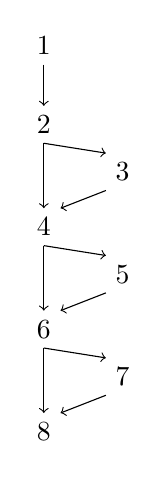
\begin{tikzpicture}[scale=0.6]
 \node[name=one] {1};
 \node[name=two, below of=one, yshift=0mm] {2};
 \node[name=three, right of=two, yshift=-6mm] {3};
 \node[name=four, below of=two, yshift=-3mm] {4};
 \node[name=five, right of=four, yshift=-6mm] {5};
 \node[name=six, below of=four, yshift=-3mm] {6};
 \node[name=seven, right of=six, yshift=-6mm] {7};
 \node[name=eight, below of=six, yshift=-3mm] {8};
 
 \draw (one.south) edge[->] (two.north);
 \draw (two.south) edge[->] (four.north);
 \draw (two.south) edge[->] (three.north west);
 \draw (three.south west) edge[->] (four.north east);
 \draw (four.south) edge[->] (six.north);
 \draw (four.south) edge[->] (five.north west);
 \draw (five.south west) edge[->] (six.north east);
 \draw (six.south) edge[->] (eight.north);
 \draw (six.south) edge[->] (seven.north west);
 \draw (seven.south west) edge[->] (eight.north east);
\end{tikzpicture}
\end{minipage}
\vfill
Is there a trace that leads to the \texttt{assert} being violated?
\end{frame}

\begin{frame}[fragile]
\frametitle{Program Analysis in a nutshell}
\vfill
Graphs can encode large sets of program traces
\pause
\begin{itemize}
\item exploit well-understood graph algorithms for analysis
\item e.g., DFS, intersection/union over prefixes/suffixes of paths, etc.
\end{itemize}
\pause
\vfill
... but they approximate the set of traces
\vfill
\begin{center}
\def\supercircle{(0,0) circle (1.25cm)}
\def\progtraces{(0:3cm) circle (1.0cm)}
\def\subcircle{(0:6cm) circle (0.75cm)}

\tikzset{red/.style={fill=red}}
\tikzset{green/.style={fill=green}}

\begin{tikzpicture}%[scale=1.0]
  \draw \progtraces node[below] {program};
  \draw[red] \supercircle node[yshift=-15mm,below] {over-approximation};
  \draw[green] \subcircle node[yshift=-15mm,below] {under-approximation};
\end{tikzpicture}
\end{center}
\vfill
\end{frame}

\begin{frame}[fragile]
\frametitle{Program Analysis in a nutshell}
\vfill
Graphs can encode large sets of program traces
\begin{itemize}
\item exploit well-understood graph algorithms for analysis
\item e.g., DFS, intersection/union over prefixes/suffixes of paths, etc.
\end{itemize}
\vfill
... but they approximate the set of traces
\begin{center}
\def\supertraces{(0,0) circle (1.0cm)}
\def\supercircle{(0,0) circle (1.25cm)}
\def\subcircle{(0:6cm) circle (0.75cm)}
\def\subtraces{(0:6cm) circle (1.0cm)}

\tikzset{red/.style={fill=red}}
\tikzset{green/.style={fill=green}}

\begin{tikzpicture}%[scale=1.0]
  \begin{scope}
     \clip \supercircle;
     \draw[red, even odd rule] \supercircle \supertraces;
  \end{scope}
  \draw\subtraces;
  \draw[green] \subcircle;
  \draw \supercircle node[yshift=-15mm,below] {extra behavior};
  \draw \subcircle node[yshift=-15mm,below] {missing behavior};
\end{tikzpicture}
\end{center}
\vfill
\end{frame}

\begin{frame}[fragile]
\frametitle{Where is the overapproximation?}
\vfill
\begin{minipage}[t]{0.4\textwidth}
\lstset{numbers=left, numbersep=2pt}
\begin{center}
\begin{lstlisting}
int classify(int a, int b, int c) {
  if (a==b) 
    type+=1;
  if (a==c) 
    type+=2;
  if (b==c) 
    type+=3;
  assert type != 6; ...
\end{lstlisting}
\end{center}
\end{minipage}
\hfill
\begin{minipage}[t]{0.4\textwidth}
A \textbf{graph} of program traces
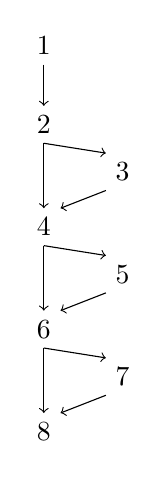
\begin{tikzpicture}[scale=0.6]
 \node[name=one] {1};
 \node[name=two, below of=one, yshift=0mm] {2};
 \node[name=three, right of=two, yshift=-6mm] {3};
 \node[name=four, below of=two, yshift=-3mm] {4};
 \node[name=five, right of=four, yshift=-6mm] {5};
 \node[name=six, below of=four, yshift=-3mm] {6};
 \node[name=seven, right of=six, yshift=-6mm] {7};
 \node[name=eight, below of=six, yshift=-3mm] {8};
 
 \draw (one.south) edge[->] (two.north);
 \draw (two.south) edge[->] (four.north);
 \draw (two.south) edge[->] (three.north west);
 \draw (three.south west) edge[->] (four.north east);
 \draw (four.south) edge[->] (six.north);
 \draw (four.south) edge[->] (five.north west);
 \draw (five.south west) edge[->] (six.north east);
 \draw (six.south) edge[->] (eight.north);
 \draw (six.south) edge[->] (seven.north west);
 \draw (seven.south west) edge[->] (eight.north east);
\end{tikzpicture}
\end{minipage}
\vfill
\end{frame}

\begin{frame}[fragile]
\frametitle{Underapproximating Symbolic Execution }
\vfill
\begin{minipage}[t]{0.4\textwidth}
\lstset{numbers=left, numbersep=2pt}
\begin{center}
\begin{lstlisting}
int classify(int a, int b, int c) {
  if (a==b) 
    type+=1;
  if (a==c) 
    type+=2;
  if (b==c) 
    type+=3;
  assert type != 6; ...
\end{lstlisting}
\end{center}
\end{minipage}
\hfill
\begin{minipage}[t]{0.4\textwidth}
A \textbf{tree} of program traces
\begin{tikzpicture}[scale=0.6, sibling distance=20pt, level distance=30pt]
 \node {1}
  child {
   node {2}
    child {
     node[xshift=-7mm] {3}
      child {
       node {4}
        child {
         node[xshift=-3mm] {5}
          child {
           node {6}
            child {
             node {7}
              child {
               node {8}
               edge from parent
              }
             edge from parent
            }
            %child {
            % node {8}
            % edge from parent
            %}
           edge from parent
          }
         edge from parent
        }
        child {
         node[xshift=3mm] {6}
          %child {
          % node {7}
          %  child {
          %   node {8}
          %   edge from parent
          %  }
          % edge from parent
          %}
          child {
           node {8}
           edge from parent
          }
         edge from parent
        }
       edge from parent
      }
     edge from parent
    }
    child {
     node[xshift=7mm] {4}
        child {
         node[xshift=-3mm] {5}
          child {
           node {6}
            %child {
            % node {7}
            %  child {
            %   node {8}
            %   edge from parent
            %  }
            % edge from parent
            %}
            child {
             node {8}
             edge from parent
            }
           edge from parent
          }
         edge from parent
        }
        child {
         node[xshift=3mm] {6}
          child {
           node {7}
            child {
             node {8}
             edge from parent
            }
           edge from parent
          }
          child {
           node {8}
           edge from parent
          }
         edge from parent
     edge from parent
    }
   edge from parent
  }
 };
\end{tikzpicture}
\end{minipage}
\vfill
\end{frame}


\begin{frame}{Basic symbolic execution algorithm} 
\begin{algorithm}[H]
\small
\caption{{\tt symbolicExecute}$(l,\phi,m)$}
\begin{algorithmic}
 \WHILE{$\neg branch(l)$}
   \STATE $m \gets m\lrangle{v, e}$
   \STATE $l \gets next(l)$
 \ENDWHILE

 \STATE $c \gets m[\x{cond}(l)]$

 \IF{SAT$(\phi \wedge c)$}
   \STATE {\tt symbolicExecute}$(\x{target}(l), \phi \wedge c, m)$
 \ENDIF

 \IF{SAT$(\phi \wedge \neg c)$}
   \STATE {\tt symbolicExecute}$(\x{next}(l), \phi \wedge \neg c, m)$
 \ENDIF
\end{algorithmic}
\end{algorithm}
\end{frame}

\begin{frame}[fragile]
\frametitle{A simple example ...}
\begin{center}
\begin{lstlisting}
int classify(int a, int b, int c) {
  if (a<=0 || b<=0 || c<=0) return 4;
  int type=0;
  if (a==b) type+=1;
  if (a==c) type+=2;
  if (b==c) type+=3;
  if (type==0) {
    if (a+b<=c || b+c<=a || a+c>=b) type=4;
    else type=1;
    return type;
  }
  if (type>3) type=3;
  else if (type==1 && a+b>c) type=2;
  else if (type==2 && a+c>b) type=2;
  else if (type==3 && b+c>a) type=2;
  else type=4;
  return type;
}
\end{lstlisting}
\end{center}
\end{frame}

\newcommand{\Hilight}{\makebox[0pt][l]{\color{yellow}\rule[-0.45em]{\linewidth}{1.5em}}}
\begin{frame}[fragile]
\frametitle{A simple example ...}
\begin{center}
\begin{lstlisting}[escapechar=\%]
int classify(int a, int b, int c) {
  %\Hilight%if (a<=0 || b<=0 || c<=0) return 4;
  int type=0;
  if (a==b) type+=1;
  if (a==c) type+=2;
  if (b==c) type+=3;
  if (type==0) {
    if (a+b<=c || b+c<=a || a+c>=b) type=4;
    else type=1;
    return type;
  }
  if (type>3) type=3;
  else if (type==1 && a+b>c) type=2;
  else if (type==2 && a+c>b) type=2;
  else if (type==3 && b+c>a) type=2;
  else type=4;
  return type;
}
\end{lstlisting}
\end{center}
\end{frame}

\begin{frame}{Symbolic execution tree}
\begin{center}
\begin{tikzpicture}[scale=0.6]
  \node {\texttt{a$\le$0}}
     child {
       node[xshift=-7mm, yshift=3mm] {\colorbox{Green}{4}}
       edge from parent
     }
     child {
       node[xshift=5mm, yshift=3mm] {$b \le 0$}
       child {
         node[xshift=-7mm, yshift=3mm] {\colorbox{Green}{4}}
         edge from parent
       }
       child {
         node[xshift=5mm, yshift=3mm] {$c \le 0$}
         child {
           node[xshift=-7mm, yshift=3mm] {\colorbox{Green}{4}}
           edge from parent
         }
         child [color=white] {
           node[xshift=5mm, yshift=3mm] {$a=b$}
           child {
             node[xshift=-30mm, yshift=2mm] {$a=c$}
             child {
               node[xshift=-4mm, yshift=3mm] {$b=c$}
               child {
                 node[xshift=0mm, yshift=2mm] {}
                 edge from parent
               }
               child {
                 node[xshift=0mm, yshift=2mm] {}
                 edge from parent
               }
               edge from parent
             }
             child {
               node[xshift=4mm, yshift=3mm] {$b=c$}
               child {
                 node[xshift=-2mm, yshift=2mm] {}
                 edge from parent
               }
               child { 
                 node[xshift=0mm, yshift=2mm] {$a+b>c$}
                 child {
                   node[yshift=2mm] {}
                   edge from parent
                 }
                 child {
                   node[yshift=2mm] {}
                   edge from parent
                 }
                 edge from parent
               }
               edge from parent
             }
             edge from parent
           }
           child {
             node[xshift=10mm, yshift=2mm] {$a=c$}
             child {
               node[xshift=-13mm, yshift=3mm] {$b=c$}
               child {
                 node[xshift=-2mm, yshift=2mm] {}
                 edge from parent
               }
               child {
                 node[xshift=0mm, yshift=2mm] {$a+c>b$}
                 child {
                   node[yshift=2mm] {}
                   edge from parent
                 }
                 child {
                   node[yshift=2mm] {}
                   edge from parent
                 }
                 edge from parent
               }
               edge from parent
             }
             child {
               node[xshift=20mm, yshift=3mm] {$b=c$}
               child {
                 node[xshift=-15mm, yshift=2mm] {$b+c>a$}
                 child {
                   node[yshift=2mm] {}
                   edge from parent
                 }
                 child {
                   node[yshift=2mm] {}
                   edge from parent
                 }
                 edge from parent
               }
               child {
                 node[xshift=0mm, yshift=2mm] {$a+b \le c$}
                 child {
                   node[xshift=-5mm, yshift=2mm] {}
                   edge from parent
                 }
                 child {
                   node[xshift=5mm, yshift=2mm] {$b+c \le a$}
                   child {
                     node[xshift=-5mm, yshift=2mm] {}
                     edge from parent
                   }
                   child {
                     node[xshift=0mm, yshift=2mm] {$a+c \ge b$}
                     child {
                       node[yshift=2mm] {}
                       edge from parent
                     }
                     child {
                       node[yshift=2mm] {}
                       edge from parent
                     }
                     edge from parent
                   }
                   edge from parent
                 }
                 edge from parent
               }
               edge from parent
             }
             edge from parent
           }
           edge from parent
         }
         edge from parent
       }
       edge from parent
     };
\end{tikzpicture}
\end{center}
\end{frame}

\begin{frame}[fragile]
\frametitle{A simple example ...}
\begin{center}
\begin{lstlisting}[escapechar=\%]
int classify(int a, int b, int c) {
  if (a<=0 || b<=0 || c<=0) return 4;
  int type=0;
  %\Hilight%if (a==b) type+=1;
  %\Hilight%if (a==c) type+=2;
  %\Hilight%if (b==c) type+=3;
  if (type==0) {
    if (a+b<=c || b+c<=a || a+c>=b) type=4;
    else type=1;
    return type;
  }
  if (type>3) type=3;
  else if (type==1 && a+b>c) type=2;
  else if (type==2 && a+c>b) type=2;
  else if (type==3 && b+c>a) type=2;
  else type=4;
  return type;
}
\end{lstlisting}
\end{center}
\end{frame}

\begin{frame}{Symbolic execution tree}
\begin{center}
\begin{tikzpicture}[scale=0.6]
  \node {\texttt{a$\le$0}}
     child {
       node[xshift=-7mm, yshift=3mm] {\colorbox{Green}{4}}
       edge from parent
     }
     child {
       node[xshift=5mm, yshift=3mm] {$b \le 0$}
       child {
         node[xshift=-7mm, yshift=3mm] {\colorbox{Green}{4}}
         edge from parent
       }
       child {
         node[xshift=5mm, yshift=3mm] {$c \le 0$}
         child {
           node[xshift=-7mm, yshift=3mm] {\colorbox{Green}{4}}
           edge from parent
         }
         child {
           node[xshift=5mm, yshift=3mm] {$a=b$}
           child {
             node[xshift=-30mm, yshift=2mm] {$a=c$}
             child {
               node[xshift=-4mm, yshift=3mm] {$b=c$}
               child [color=white] {
                 node[xshift=0mm, yshift=2mm] {}
                 edge from parent
               }
               child [color=white] {
                 node[xshift=0mm, yshift=2mm] {}
                 edge from parent
               }
               edge from parent
             }
             child {
               node[xshift=4mm, yshift=3mm] {$b=c$}
               child [color=white] {
                 node[xshift=-2mm, yshift=2mm] {}
                 edge from parent
               }
               child [color=white] { 
                 node[xshift=0mm, yshift=2mm] {$a+b>c$}
                 child {
                   node[yshift=2mm] {}
                   edge from parent
                 }
                 child {
                   node[yshift=2mm] {}
                   edge from parent
                 }
                 edge from parent
               }
               edge from parent
             }
             edge from parent
           }
           child {
             node[xshift=10mm, yshift=2mm] {$a=c$}
             child {
               node[xshift=-13mm, yshift=3mm] {$b=c$}
               child [color=white] {
                 node[xshift=-2mm, yshift=2mm] {}
                 edge from parent
               }
               child [color=white] {
                 node[xshift=0mm, yshift=2mm] {$a+c>b$}
                 child {
                   node[yshift=2mm] {}
                   edge from parent
                 }
                 child {
                   node[yshift=2mm] {}
                   edge from parent
                 }
                 edge from parent
               }
               edge from parent
             }
             child {
               node[xshift=20mm, yshift=3mm] {$b=c$}
               child [color=white] {
                 node[xshift=-15mm, yshift=2mm] {$b+c>a$}
                 child {
                   node[yshift=2mm] {}
                   edge from parent
                 }
                 child {
                   node[yshift=2mm] {}
                   edge from parent
                 }
                 edge from parent
               }
               child [color=white] {
                 node[xshift=0mm, yshift=2mm] {$a+b \le c$}
                 child {
                   node[xshift=-5mm, yshift=2mm] {}
                   edge from parent
                 }
                 child {
                   node[xshift=5mm, yshift=2mm] {$b+c \le a$}
                   child {
                     node[xshift=-5mm, yshift=2mm] {}
                     edge from parent
                   }
                   child {
                     node[xshift=0mm, yshift=2mm] {$a+c \ge b$}
                     child {
                       node[yshift=2mm] {}
                       edge from parent
                     }
                     child {
                       node[yshift=2mm] {}
                       edge from parent
                     }
                     edge from parent
                   }
                   edge from parent
                 }
                 edge from parent
               }
               edge from parent
             }
             edge from parent
           }
           edge from parent
         }
         edge from parent
       }
       edge from parent
     };
\end{tikzpicture}
\end{center}
\end{frame}

\begin{frame}[fragile]
\frametitle{A simple example ...}
\begin{center}
\begin{lstlisting}[escapechar=\%]
int classify(int a, int b, int c) {
  if (a<=0 || b<=0 || c<=0) return 4;
  int type=0;
  if (a==b) type+=1;
  if (a==c) type+=2;
  if (b==c) type+=3;
  if (type==0) {
    if (a+b<=c || b+c<=a || a+c>=b) type=4;
    else type=1;
    return type;
  }
  %\Hilight%if (type>3) type=3;
  %\Hilight%else if (type==1 && a+b>c) type=2;
  %\Hilight%else if (type==2 && a+c>b) type=2;
  %\Hilight%else if (type==3 && b+c>a) type=2;
  %\Hilight%else type=4;
  return type;
}
\end{lstlisting}
\end{center}
\end{frame}

\begin{frame}{Symbolic execution tree}
\begin{center}
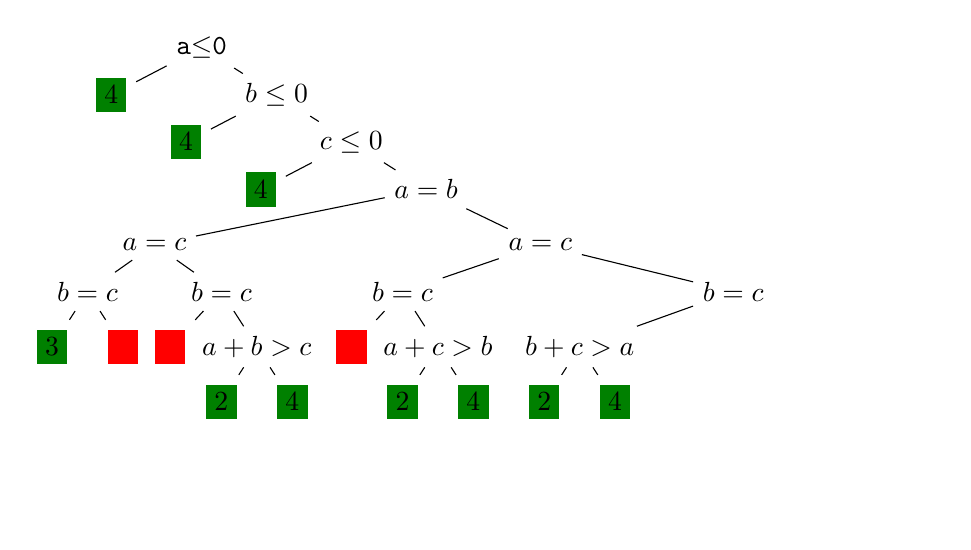
\begin{tikzpicture}[scale=0.6]
  \node {\texttt{a$\le$0}}
     child [color=black] {
       node[xshift=-7mm, yshift=3mm] {\colorbox{Green}{4}}
       edge from parent
     }
     child [color=black] {
       node[xshift=5mm, yshift=3mm] {$b \le 0$}
       child {
         node[xshift=-7mm, yshift=3mm] {\colorbox{Green}{4}}
         edge from parent
       }
       child {
         node[xshift=5mm, yshift=3mm] {$c \le 0$}
         child {
           node[xshift=-7mm, yshift=3mm] {\colorbox{Green}{4}}
           edge from parent
         }
         child {
           node[xshift=5mm, yshift=3mm] {$a=b$}
           child {
             node[xshift=-30mm, yshift=2mm] {$a=c$}
             child {
               node[xshift=-4mm, yshift=3mm] {$b=c$}
               child {
                 node[xshift=0mm, yshift=2mm] {\colorbox{Green}{3}}
                 edge from parent
               }
               child {
                 node[xshift=0mm, yshift=2mm] {\colorbox{Red}{\textcolor{Red}{3}}}
                 edge from parent
               }
               edge from parent
             }
             child {
               node[xshift=4mm, yshift=3mm] {$b=c$}
               child {
                 node[xshift=-2mm, yshift=2mm] {\colorbox{Red}{\textcolor{Red}{3}}}
                 edge from parent
               }
               child { 
                 node[xshift=0mm, yshift=2mm] {$a+b>c$}
                 child {
                   node[yshift=2mm] {\colorbox{Green}{2}}
                   edge from parent
                 }
                 child {
                   node[yshift=2mm] {\colorbox{Green}{4}}
                   edge from parent
                 }
                 edge from parent
               }
               edge from parent
             }
             edge from parent
           }
           child {
             node[xshift=10mm, yshift=2mm] {$a=c$}
             child {
               node[xshift=-13mm, yshift=3mm] {$b=c$}
               child {
                 node[xshift=-2mm, yshift=2mm] {\colorbox{Red}{\textcolor{Red}{3}}}
                 edge from parent
               }
               child {
                 node[xshift=0mm, yshift=2mm] {$a+c>b$}
                 child {
                   node[yshift=2mm] {\colorbox{Green}{2}}
                   edge from parent
                 }
                 child {
                   node[yshift=2mm] {\colorbox{Green}{4}}
                   edge from parent
                 }
                 edge from parent
               }
               edge from parent
             }
             child {
               node[xshift=20mm, yshift=3mm] {$b=c$}
               child {
                 node[xshift=-15mm, yshift=2mm] {$b+c>a$}
                 child {
                   node[yshift=2mm] {\colorbox{Green}{2}}
                   edge from parent
                 }
                 child {
                   node[yshift=2mm] {\colorbox{Green}{4}}
                   edge from parent
                 }
                 edge from parent
               }
               child [color=white] {
                 node[xshift=0mm, yshift=2mm] {$a+b \le c$}
                 child {
                   node[xshift=-5mm, yshift=2mm] {}
                   edge from parent
                 }
                 child {
                   node[xshift=5mm, yshift=2mm] {$b+c \le a$}
                   child {
                     node[xshift=-5mm, yshift=2mm] {}
                     edge from parent
                   }
                   child {
                     node[xshift=0mm, yshift=2mm] {$a+c \ge b$}
                     child {
                       node[yshift=2mm] {}
                       edge from parent
                     }
                     child {
                       node[yshift=2mm] {}
                       edge from parent
                     }
                     edge from parent
                   }
                   edge from parent
                 }
                 edge from parent
               }
               edge from parent
             }
             edge from parent
           }
           edge from parent
         }
         edge from parent
       }
       edge from parent
     };
\end{tikzpicture}
\end{center}
\end{frame}

\begin{frame}[fragile]
\frametitle{A simple example ...}
\begin{center}
\begin{lstlisting}[escapechar=\%]
int classify(int a, int b, int c) {
  if (a<=0 || b<=0 || c<=0) return 4;
  int type=0;
  if (a==b) type+=1;
  if (a==c) type+=2;
  if (b==c) type+=3;
  if (type==0) {
    %\Hilight%if (a+b<=c || b+c<=a || a+c>=b) type=4;
    %\Hilight%else type=1;
    %\Hilight%return type;
  }
  if (type>3) type=3;
  else if (type==1 && a+b>c) type=2;
  else if (type==2 && a+c>b) type=2;
  else if (type==3 && b+c>a) type=2;
  else type=4;
  return type;
}
\end{lstlisting}
\end{center}
\end{frame}

\begin{frame}{Symbolic execution tree}
\begin{center}
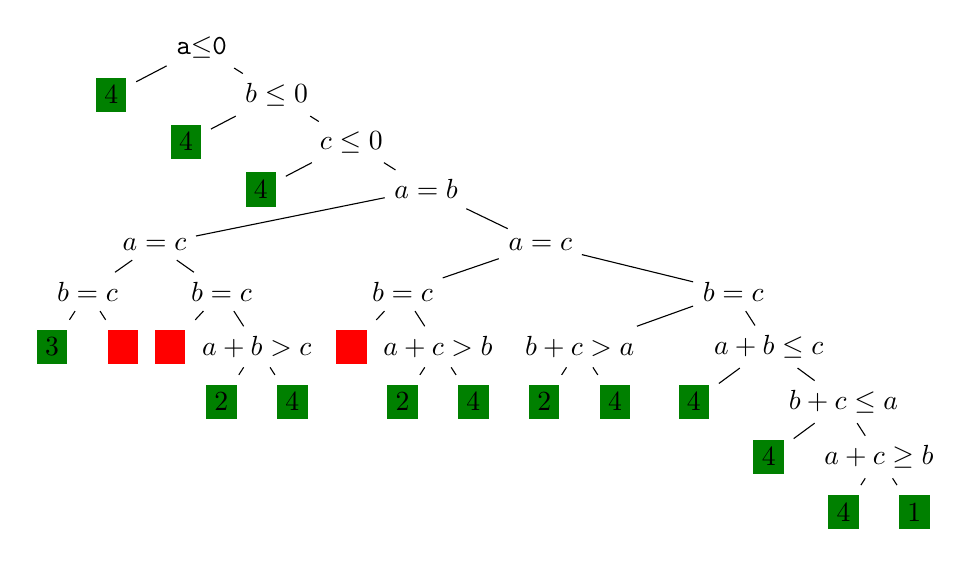
\begin{tikzpicture}[scale=0.6]
  \node {\texttt{a$\le$0}}
     child [color=black] {
       node[xshift=-7mm, yshift=3mm] {\colorbox{Green}{4}}
       edge from parent
     }
     child [color=black] {
       node[xshift=5mm, yshift=3mm] {$b \le 0$}
       child {
         node[xshift=-7mm, yshift=3mm] {\colorbox{Green}{4}}
         edge from parent
       }
       child {
         node[xshift=5mm, yshift=3mm] {$c \le 0$}
         child {
           node[xshift=-7mm, yshift=3mm] {\colorbox{Green}{4}}
           edge from parent
         }
         child {
           node[xshift=5mm, yshift=3mm] {$a=b$}
           child {
             node[xshift=-30mm, yshift=2mm] {$a=c$}
             child {
               node[xshift=-4mm, yshift=3mm] {$b=c$}
               child {
                 node[xshift=0mm, yshift=2mm] {\colorbox{Green}{3}}
                 edge from parent
               }
               child {
                 node[xshift=0mm, yshift=2mm] {\colorbox{Red}{\textcolor{Red}{3}}}
                 edge from parent
               }
               edge from parent
             }
             child {
               node[xshift=4mm, yshift=3mm] {$b=c$}
               child {
                 node[xshift=-2mm, yshift=2mm] {\colorbox{Red}{\textcolor{Red}{3}}}
                 edge from parent
               }
               child { 
                 node[xshift=0mm, yshift=2mm] {$a+b>c$}
                 child {
                   node[yshift=2mm] {\colorbox{Green}{2}}
                   edge from parent
                 }
                 child {
                   node[yshift=2mm] {\colorbox{Green}{4}}
                   edge from parent
                 }
                 edge from parent
               }
               edge from parent
             }
             edge from parent
           }
           child {
             node[xshift=10mm, yshift=2mm] {$a=c$}
             child {
               node[xshift=-13mm, yshift=3mm] {$b=c$}
               child {
                 node[xshift=-2mm, yshift=2mm] {\colorbox{Red}{\textcolor{Red}{3}}}
                 edge from parent
               }
               child {
                 node[xshift=0mm, yshift=2mm] {$a+c>b$}
                 child {
                   node[yshift=2mm] {\colorbox{Green}{2}}
                   edge from parent
                 }
                 child {
                   node[yshift=2mm] {\colorbox{Green}{4}}
                   edge from parent
                 }
                 edge from parent
               }
               edge from parent
             }
             child {
               node[xshift=20mm, yshift=3mm] {$b=c$}
               child {
                 node[xshift=-15mm, yshift=2mm] {$b+c>a$}
                 child {
                   node[yshift=2mm] {\colorbox{Green}{2}}
                   edge from parent
                 }
                 child {
                   node[yshift=2mm] {\colorbox{Green}{4}}
                   edge from parent
                 }
                 edge from parent
               }
               child {
                 node[xshift=0mm, yshift=2mm] {$a+b \le c$}
                 child {
                   node[xshift=-5mm, yshift=2mm] {\colorbox{Green}{4}}
                   edge from parent
                 }
                 child {
                   node[xshift=5mm, yshift=2mm] {$b+c \le a$}
                   child {
                     node[xshift=-5mm, yshift=2mm] {\colorbox{Green}{4}}
                     edge from parent
                   }
                   child {
                     node[xshift=0mm, yshift=2mm] {$a+c \ge b$}
                     child {
                       node[yshift=2mm] {\colorbox{Green}{4}}
                       edge from parent
                     }
                     child {
                       node[yshift=2mm] {\colorbox{Green}{1}}
                       edge from parent
                     }
                     edge from parent
                   }
                   edge from parent
                 }
                 edge from parent
               }
               edge from parent
             }
             edge from parent
           }
           edge from parent
         }
         edge from parent
       }
       edge from parent
     };
\end{tikzpicture}
\end{center}
\end{frame}

\begin{frame}{Some observations}
\vfill
\begin{itemize}
\item There are 14 distinct paths (Green): from 1 to 9 branches
\vfill
\item 1 path returns ``scalene'' (1); 3 return ``isoscelese'' (2); and 1 returns ``equilateral'' (3)
\vfill
\item 3 paths are pruned because constraints are unsat (Red)
\vfill
\item Interesting symmetries are involved in the ``isoscelese'' and unsat cases
\end{itemize}
\vfill
\end{frame}

\begin{frame}{Analyzing program behavior}
\vfill
The symbolic execution could be used to ...
\begin{itemize}
\vfill
\item check contracts, e.g., if $a=b=c$ then $return=3$
\vfill
\item generate a suite of 14 thorough tests
\vfill
\item demonstrate that it is possible to return values $[1,4]$
\vfill
\end{itemize}
... and support answering other yes/no questions about program behavior.
\vfill
\end{frame}

\begin{frame}{Moving beyond yes/no questions}
\vfill
We are interested in exploring how to ...
\vfill
\begin{itemize}
\item determine the chance that a contract holds (1 is a special case)
\vfill
\item focus testing on {\em rare} paths (likely ones are easy to hit)
\vfill
\item determine how frequently a given value is returned
\end{itemize}
\vfill
\pause
When yes/no questions cannot be answered can we quantify what
was discovered during program analysis?
\vfill
\end{frame}

\begin{frame}{Assume \texttt{int}s are drawn uniformly from $[-1000,1000]$}
\begin{center}
\pgfdeclarelayer{foreground}
\pgfsetlayers{main,foreground}
\begin{tikzpicture}[scale=0.6]
  \node {\texttt{a$\le$0}}
     child [color=black] {
       node[xshift=-7mm, yshift=3mm] {\colorbox{Green}{4}}
       edge from parent
     }
     child [color=black] {
       node[xshift=5mm, yshift=3mm] {$b \le 0$}
       child {
         node[xshift=-7mm, yshift=3mm] {\colorbox{Green}{4}}
         edge from parent
       }
       child {
         node[xshift=5mm, yshift=3mm] {$c \le 0$}
         child {
           node[xshift=-7mm, yshift=3mm] {\colorbox{Green}{4}}
           edge from parent
         }
         child {
           node[name=reference, xshift=5mm, yshift=3mm] {$a=b$}
           child {
             node[xshift=-30mm, yshift=2mm] {$a=c$}
             child {
               node[xshift=-4mm, yshift=3mm] {$b=c$}
               child {
                 node[xshift=0mm, yshift=2mm] {\colorbox{Green}{3}}
                 edge from parent
               }
               child {
                 node[xshift=0mm, yshift=2mm] {\colorbox{Red}{\textcolor{Red}{3}}}
                 edge from parent
               }
               edge from parent
             }
             child {
               node[xshift=4mm, yshift=3mm] {$b=c$}
               child {
                 node[xshift=-2mm, yshift=2mm] {\colorbox{Red}{\textcolor{Red}{3}}}
                 edge from parent
               }
               child { 
                 node[xshift=0mm, yshift=2mm] {$a+b>c$}
                 child {
                   node[yshift=2mm] {\colorbox{Green}{2}}
                   edge from parent
                 }
                 child {
                   node[yshift=2mm] {\colorbox{Green}{4}}
                   edge from parent
                 }
                 edge from parent
               }
               edge from parent
             }
             edge from parent
           }
           child {
             node[xshift=10mm, yshift=2mm] {$a=c$}
             child {
               node[xshift=-13mm, yshift=3mm] {$b=c$}
               child {
                 node[xshift=-2mm, yshift=2mm] {\colorbox{Red}{\textcolor{Red}{3}}}
                 edge from parent
               }
               child {
                 node[xshift=0mm, yshift=2mm] {$a+c>b$}
                 child {
                   node[yshift=2mm] {\colorbox{Green}{2}}
                   edge from parent
                 }
                 child {
                   node[yshift=2mm] {\colorbox{Green}{4}}
                   edge from parent
                 }
                 edge from parent
               }
               edge from parent
             }
             child {
               node[xshift=20mm, yshift=3mm] {$b=c$}
               child {
                 node[xshift=-15mm, yshift=2mm] {$b+c>a$}
                 child {
                   node[yshift=2mm] {\colorbox{Green}{2}}
                   edge from parent
                 }
                 child {
                   node[yshift=2mm] {\colorbox{Green}{4}}
                   edge from parent
                 }
                 edge from parent
               }
               child {
                 node[xshift=0mm, yshift=2mm] {$a+b \le c$}
                 child {
                   node[xshift=-5mm, yshift=2mm] {\colorbox{Green}{4}}
                   edge from parent
                 }
                 child {
                   node[xshift=5mm, yshift=2mm] {$b+c \le a$}
                   child {
                     node[xshift=-5mm, yshift=2mm] {\colorbox{Green}{4}}
                     edge from parent
                   }
                   child {
                     node[xshift=0mm, yshift=2mm] {$a+c \ge b$}
                     child {
                       node[yshift=2mm] {\colorbox{Green}{4}}
                       edge from parent
                     }
                     child {
                       node[yshift=2mm] {\colorbox{Green}{1}}
                       edge from parent
                     }
                     edge from parent
                   }
                   edge from parent
                 }
                 edge from parent
               }
               edge from parent
             }
             edge from parent
           }
           edge from parent
         }
         edge from parent
       }
       edge from parent
     };

   \begin{pgfonlayer}{foreground}
      \node[name=first, xshift=30mm, yshift=6mm, above of=reference] 
         {\large Likelihood that \texttt{classify} returns equilateral?}; 
   \end{pgfonlayer}

\end{tikzpicture}
\end{center}
\end{frame}

\begin{frame}{Assume \texttt{int}s are drawn uniformly from $[-1000,1000]$}
\begin{center}
\pgfdeclarelayer{foreground}
\pgfsetlayers{main,foreground}
\begin{tikzpicture}[scale=0.6]
  \node {\texttt{a$\le$0}}
     child [color=white] {
       node[xshift=-7mm, yshift=3mm] {}
       edge from parent
     }
     child {
       node[xshift=5mm, yshift=3mm] {$b \le 0$}
       child [color=white] {
         node[xshift=-7mm, yshift=3mm] {}
         edge from parent
       }
       child {
         node[xshift=5mm, yshift=3mm] {$c \le 0$}
         child [color=white] {
           node[xshift=-7mm, yshift=3mm] {}
           edge from parent
         }
         child {
           node[name=reference, xshift=5mm, yshift=3mm] {$a=b$}
           child {
             node[xshift=-30mm, yshift=2mm] {$a=c$}
             child {
               node[xshift=-4mm, yshift=3mm] {$b=c$}
               child {
                 node[name=ref2, xshift=0mm, yshift=2mm] {\colorbox{Green}{3}}
                 edge from parent
               }
               child [color=white]{
                 node[xshift=0mm, yshift=2mm] {}
                 edge from parent
               }
               edge from parent
             }
             child [color=white] {
               node[xshift=4mm, yshift=3mm] {$b=c$}
               child {
                 node[xshift=-2mm, yshift=2mm] {}
                 edge from parent
               }
               child { 
                 node[xshift=0mm, yshift=2mm] {$a+b>c$}
                 child {
                   node[yshift=2mm] {}
                   edge from parent
                 }
                 child {
                   node[yshift=2mm] {}
                   edge from parent
                 }
                 edge from parent
               }
               edge from parent
             }
             edge from parent
           }
           child [color=white] {
             node[xshift=10mm, yshift=2mm] {$a=c$}
             child [color=white] {
               node[xshift=-13mm, yshift=3mm] {$b=c$}
               child {
                 node[xshift=-2mm, yshift=2mm] {}
                 edge from parent
               }
               child {
                 node[xshift=0mm, yshift=2mm] {$a+c>b$}
                 child {
                   node[yshift=2mm] {}
                   edge from parent
                 }
                 child {
                   node[yshift=2mm] {}
                   edge from parent
                 }
                 edge from parent
               }
               edge from parent
             }
             child {
               node[xshift=20mm, yshift=3mm] {$b=c$}
               child [color=white] {
                 node[xshift=-15mm, yshift=2mm] {$b+c>a$}
                 child {
                   node[yshift=2mm] {}
                   edge from parent
                 }
                 child {
                   node[yshift=2mm] {}
                   edge from parent
                 }
                 edge from parent
               }
               child {
                 node[xshift=0mm, yshift=2mm] {$a+b \le c$}
                 child {
                   node[xshift=-5mm, yshift=2mm] {}
                   edge from parent
                 }
                 child {
                   node[xshift=5mm, yshift=2mm] {$b+c \le a$}
                   child {
                     node[xshift=-5mm, yshift=2mm] {}
                     edge from parent
                   }
                   child {
                     node[xshift=0mm, yshift=2mm] {$a+c \ge b$}
                     child {
                       node[yshift=2mm] {}
                       edge from parent
                     }
                     child {
                       node[yshift=2mm] {}
                       edge from parent
                     }
                     edge from parent
                   }
                   edge from parent
                 }
                 edge from parent
               }
               edge from parent
             }
             edge from parent
           }
           edge from parent
         }
         edge from parent
       }
       edge from parent
     };

   \begin{pgfonlayer}{foreground}
      \node[name=first, xshift=30mm, yshift=6mm, above of=reference] 
         {\large Likelihood that \texttt{classify} returns equilateral?}; 
       \pause
       \node[name=pc, right of=ref2, xshift=40mm] 
          {$\neg(a\le0) \wedge \neg(b\le0) \wedge \neg(c\le0) \wedge (a=b) \wedge (a=c) \wedge (b=c)$}; 
       \pause
       \node[name=question, below of=pc] 
          {How many inputs satisfy this path condition?};
       \pause
       \node[name=answer, below of=question] 
          {1000};
       \pause
       \node[name=firstanswer, below of=first] 
          {$1.25e^{-7}$};
   \end{pgfonlayer}

\end{tikzpicture}
\end{center}
\end{frame}

\ignore{
\begin{frame}{Assume \texttt{int}s are drawn uniformly from $[-1000,1000]$}
\begin{center}
\pgfdeclarelayer{foreground}
\pgfsetlayers{main,foreground}
\begin{tikzpicture}[scale=0.6]
  \node {\texttt{a$\le$0}}
     child [color=white] {
       node[xshift=-7mm, yshift=3mm] {}
       edge from parent
     }
     child [color=black] {
       node[xshift=5mm, yshift=3mm] {$b \le 0$}
       child [color=white] {
         node[xshift=-7mm, yshift=3mm] {}
         edge from parent
       }
       child {
         node[xshift=5mm, yshift=3mm] {$c \le 0$}
         child [color=white] {
           node[xshift=-7mm, yshift=3mm] {}
           edge from parent
         }
         child {
           node[name=reference, xshift=5mm, yshift=3mm] {$a=b$}
           child {
             node[xshift=-30mm, yshift=2mm] {$a=c$}
             child [color=white] {
               node[xshift=-4mm, yshift=3mm] {$b=c$}
               child {
                 node[xshift=0mm, yshift=2mm] {}
                 edge from parent
               }
               child {
                 node[xshift=0mm, yshift=2mm] {}
                 edge from parent
               }
               edge from parent
             }
             child {
               node[xshift=4mm, yshift=3mm] {$b=c$}
               child [color=white] {
                 node[xshift=-2mm, yshift=2mm] {}
                 edge from parent
               }
               child { 
                 node[xshift=0mm, yshift=2mm] {$a+b>c$}
                 child {
                   node[yshift=2mm] {\colorbox{Green}{2}}
                   edge from parent
                 }
                 child [color=white] {
                   node[yshift=2mm] {}
                   edge from parent
                 }
                 edge from parent
               }
               edge from parent
             }
             edge from parent
           }
           child {
             node[xshift=10mm, yshift=2mm] {$a=c$}
             child {
               node[xshift=-13mm, yshift=3mm] {$b=c$}
               child [color=white] {
                 node[xshift=-2mm, yshift=2mm] {}
                 edge from parent
               }
               child {
                 node[xshift=0mm, yshift=2mm] {$a+c>b$}
                 child {
                   node[yshift=2mm] {\colorbox{Green}{2}}
                   edge from parent
                 }
                 child [color=white] {
                   node[yshift=2mm] {}
                   edge from parent
                 }
                 edge from parent
               }
               edge from parent
             }
             child {
               node[xshift=20mm, yshift=3mm] {$b=c$}
               child {
                 node[xshift=-15mm, yshift=2mm] {$b+c>a$}
                 child {
                   node[yshift=2mm] {\colorbox{Green}{2}}
                   edge from parent
                 }
                 child [color=white] {
                   node[yshift=2mm] {}
                   edge from parent
                 }
                 edge from parent
               }
               child [color=white] {
                 node[xshift=0mm, yshift=2mm] {$a+b \le c$}
                 child {
                   node[xshift=-5mm, yshift=2mm] {}
                   edge from parent
                 }
                 child {
                   node[xshift=5mm, yshift=2mm] {$b+c \le a$}
                   child {
                     node[xshift=-5mm, yshift=2mm] {}
                     edge from parent
                   }
                   child {
                     node[xshift=0mm, yshift=2mm] {$a+c \ge b$}
                     child {
                       node[yshift=2mm] {}
                       edge from parent
                     }
                     child {
                       node[yshift=2mm] {}
                       edge from parent
                     }
                     edge from parent
                   }
                   edge from parent
                 }
                 edge from parent
               }
               edge from parent
             }
             edge from parent
           }
           edge from parent
         }
         edge from parent
       }
       edge from parent
     };

   \begin{pgfonlayer}{foreground}
      \node[name=first, xshift=30mm, yshift=6mm, above of=reference] 
         {\large Likelihood that \texttt{classify} returns isosceles?}; \pause
      \node[name=first, below of=first] 
         {$2.80e^{-4}$}; 
   \end{pgfonlayer}

\end{tikzpicture}
\end{center}
\end{frame}
}

\begin{frame}{Some observations}
\vfill
\begin{itemize}
\item You may be able to calculate these probabilities because you know about triangles.
\pause
\vfill
\item We want to calculate the probability that a program's execution ...
\begin{itemize}
\item returns a value, reaches a statement, ...
\end{itemize}
\vfill
\pause
\item Adapting symbolic execution to perform these computations involves ...
\begin{itemize}
\item calculating the paths of interest
\item calculating the probability of taking those paths
\item combining those probabilities appropriately
\end{itemize}
\end{itemize}
\vfill
\end{frame}

\begin{frame}{Probabilistic symbolic execution algorithm} 
\begin{algorithm}[H]
\small
\caption{{\tt probSymbolicExecute}$(l,\phi,m,\colorbox{yellow}{p})$}
\begin{algorithmic}
 \WHILE{$\neg branch(l)$}
   \STATE $m \gets m\lrangle{v, e}$
   \STATE $l \gets next(l)$
 \ENDWHILE

 \STATE $c \gets m[\x{cond}(l)]$

%pr(b | p) = pr(b & p) / pr(p)
%pr(b | m) = pr(b & m) / pr(m)

 \STATE \colorbox{yellow}{$\phi' \gets \x{slice}(\phi, c)$}
 \STATE \colorbox{yellow}{$p_c \gets \x{prob}(\phi' \land c) /\x{prob}(\phi')$}

 \IF{\colorbox{yellow}{$p_c > 0$}}
   \STATE {\tt probSymbolicExecute}$(target(l), \phi \wedge c, m,$\colorbox{yellow}{$p*p_c$}$)$
 \ENDIF

 \IF{\colorbox{yellow}{$p_c < 1$}}
   \STATE {\tt probSymbolicExecute}$(next(l), \phi \wedge \neg c, m,$\colorbox{yellow}{$p*(1-p_c)$}$)$
 \ENDIF
\end{algorithmic}
\end{algorithm}
\end{frame}

\begin{frame}{Key algorithmic features}
\vfill
Slicing the path condition, i.e., $\x{slice}(\phi,c)$
\begin{itemize}
\item reduces formula size which reduces cost of $\x{prob}(\cdot)$
\item exposes opportunities for reusing computation in $\x{prob}(\cdot)$
\end{itemize}
\pause
\vfill
Calculating the conditional probability $p_c$ of $c$
\begin{itemize}
\item requires model counting of path condition
\item determines satisfiability of branches, i.e., $p_c > 0 \implies SAT(\phi \wedge c)$
\item allows inference of off-branch probability, i.e., $p*(1-p_c)$
\item depth-first nature of symbolic execution ensures that $prob(\phi')$ will be reused
\item slicing assures independence in computing $p_c$, i.e., $\phi-\phi'$ factored out
\end{itemize}
\pause
\vfill
This allows the algorithm to compute path probabilities cost-effectively.
\vfill
\end{frame}


%% in the following include the probabilities
%%   - Cyan ones are inferred (negated branch)
%%   - Orange ones are computed from reused prob(.) calls

\begin{frame}{Probabilistic symbolic execution tree}
\begin{center}
\pgfdeclarelayer{foreground}
\pgfsetlayers{main,foreground}
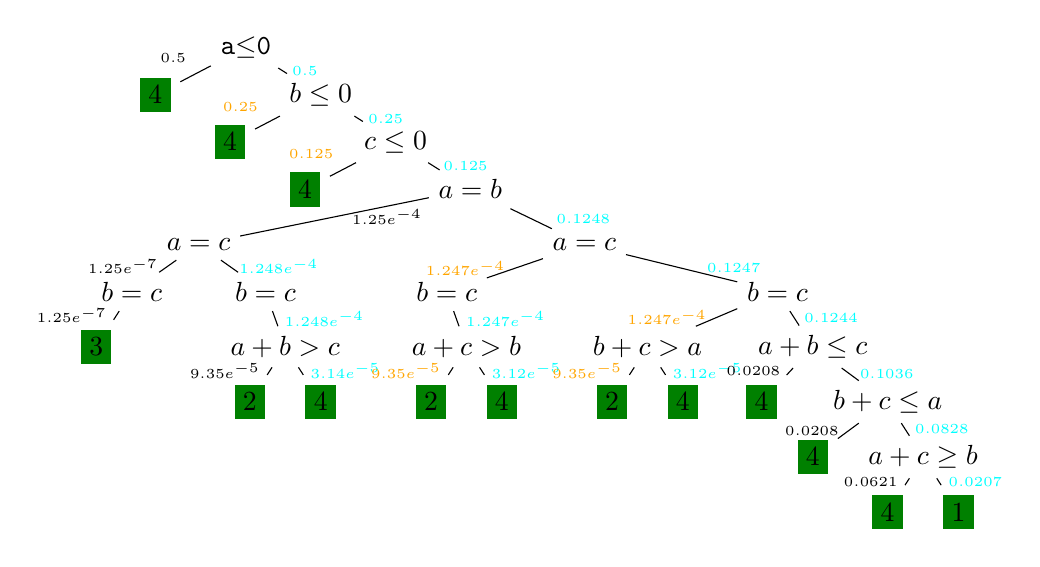
\begin{tikzpicture}[scale=0.6]
  \node {\texttt{a$\le$0}}
     child [color=black] {
       node[xshift=-7mm, yshift=3mm] {\colorbox{Green}{4}}
       edge from parent
       node[left, yshift=2mm] {\tiny $0.5$}
     }
     child [color=black] {
       node[xshift=5mm, yshift=3mm] {$b \le 0$}
       child {
         node[xshift=-7mm, yshift=3mm] {\colorbox{Green}{4}}
         edge from parent
         node[left, yshift=2mm] {\tiny \color{Orange}{$0.25$}}
       }
       child {
         node[xshift=5mm, yshift=3mm] {$c \le 0$}
         child {
           node[xshift=-7mm, yshift=3mm] {\colorbox{Green}{4}}
           edge from parent
           node[left, yshift=2mm] {\tiny \color{Orange}{$0.125$}}
         }
         child {
           node[xshift=5mm, yshift=3mm] {$a=b$}
           child {
             node[xshift=-30mm, yshift=2mm] {$a=c$}
             child {
               node[xshift=-4mm, yshift=3mm] {$b=c$}
               child {
                 node[xshift=0mm, yshift=2mm] {\colorbox{Green}{3}}
                 edge from parent
                 node[left] {\tiny $1.25e^{-7}$}
               }
               child [color=white] {
                 node[xshift=0mm, yshift=2mm] {\colorbox{white}{\textcolor{white}{3}}}
                 edge from parent
               }
               edge from parent
               node[left] {\tiny $1.25e^{-7}$}
             }
             child {
               node[xshift=4mm, yshift=3mm] {$b=c$}
               child [color=white] {
                 node[xshift=-2mm, yshift=2mm] {\colorbox{white}{\textcolor{white}{3}}}
                 edge from parent
               }
               child { 
                 node[xshift=-2mm, yshift=2mm] {$a+b>c$}
                 child {
                   node[yshift=2mm] {\colorbox{Green}{2}}
                   edge from parent
                   node[left] {\tiny $9.35e^{-5}$}
                 }
                 child {
                   node[yshift=2mm] {\colorbox{Green}{4}}
                   edge from parent
                   node[right] {\tiny \color{Cyan}{$3.14e^{-5}$}}
                 }
                 edge from parent
                 node[right] {\tiny \color{Cyan}{$1.248e^{-4}$}}
               }
               edge from parent
               node[right] {\tiny \color{Cyan}{$1.248e^{-4}$}}
             }
             edge from parent
             node[right, xshift=1mm] {\tiny {$1.25e^{-4}$}}
           }
           child {
             node[xshift=10mm, yshift=2mm] {$a=c$}
             child {
               node[xshift=-13mm, yshift=3mm] {$b=c$}
               child [color=white] {
                 node[xshift=-2mm, yshift=2mm] {\colorbox{white}{\textcolor{white}{3}}}
                 edge from parent
               }
               child {
                 node[xshift=-2mm, yshift=2mm] {$a+c>b$}
                 child {
                   node[yshift=2mm] {\colorbox{Green}{2}}
                   edge from parent
                   node[left] {\tiny \color{Orange}{$9.35e^{-5}$}}
                 }
                 child {
                   node[yshift=2mm] {\colorbox{Green}{4}}
                   edge from parent
                   node[right] {\tiny \color{Cyan}{$3.12e^{-5}$}}
                 }
                 edge from parent
                 node[right] {\tiny \color{Cyan}{$1.247e^{-4}$}}
               }
               edge from parent
               node[left] {\tiny \color{Orange}{$1.247e^{-4}$}}
             }
             child {
               node[xshift=20mm, yshift=3mm] {$b=c$}
               child {
                 node[xshift=-12mm, yshift=2mm] {$b+c>a$}
                 child {
                   node[yshift=2mm] {\colorbox{Green}{2}}
                   edge from parent
                   node[left] {\tiny \color{Orange}{$9.35e^{-5}$}}
                 }
                 child {
                   node[yshift=2mm] {\colorbox{Green}{4}}
                   edge from parent
                   node[right] {\tiny \color{Cyan}{$3.12e^{-5}$}}
                 }
                 edge from parent
               node[left] {\tiny \color{Orange}{$1.247e^{-4}$}}
               }
               child {
                 node[xshift=0mm, yshift=2mm] {$a+b \le c$}
                 child {
                   node[xshift=-2mm, yshift=2mm] {\colorbox{Green}{4}}
                   edge from parent
                   node[left] {\tiny $0.0208$}
                 }
                 child {
                   node[xshift=5mm, yshift=2mm] {$b+c \le a$}
                   child {
                     node[xshift=-5mm, yshift=2mm] {\colorbox{Green}{4}}
                     edge from parent
                     node[left] {\tiny $0.0208$}
                   }
                   child {
                     node[xshift=0mm, yshift=2mm] {$a+c \ge b$}
                     child {
                       node[yshift=2mm] {\colorbox{Green}{4}}
                       edge from parent
                       node[left] {\tiny $0.0621$}
                     }
                     child {
                       node[yshift=2mm] {\colorbox{Green}{1}}
                       edge from parent
                       node[right] {\tiny \color{Cyan}{$0.0207$}}
                     }
                     edge from parent
                     node[right] {\tiny \color{Cyan}{$0.0828$}}
                   }
                   edge from parent
                   node[right] {\tiny \color{Cyan}{$0.1036$}}
                 }
                 edge from parent
                 node[right] {\tiny \color{Cyan}{$0.1244$}}
               }
               edge from parent
               node[right,xshift=2mm] {\tiny \color{Cyan}{$0.1247$}}
             }
             edge from parent
             node[right,xshift=2mm] {\tiny \color{Cyan}{$0.1248$}}
           }
           edge from parent
           node[right] {\tiny \color{Cyan}{$0.125$}}
         }
         edge from parent
         node[right] {\tiny \color{Cyan}{$0.25$}}
       }
       edge from parent
       node[right] {\tiny \color{Cyan}{$0.5$}}
     };
\end{tikzpicture}
\end{center}

29 branches: 8 counting queries, \color{Orange}{6 reused}, \color{Cyan}{15 inferred}
\end{frame}

\begin{frame}{Probabilistic symbolic execution tree}
\begin{center}
\pgfdeclarelayer{foreground}
\pgfsetlayers{main,foreground}
\begin{tikzpicture}[scale=0.6]
  \node {\texttt{a$\le$0}}
     child [color=black] {
       node[xshift=-7mm, yshift=3mm] {\colorbox{Green}{4}}
       edge from parent
       node[left, yshift=2mm] {\tiny $0.5$}
     }
     child [color=black] {
       node[xshift=5mm, yshift=3mm] {$b \le 0$}
       child {
         node[xshift=-7mm, yshift=3mm] {\colorbox{Green}{4}}
         edge from parent
         node[left, yshift=2mm] {\tiny \color{Orange}{$0.25$}}
       }
       child {
         node[xshift=5mm, yshift=3mm] {$c \le 0$}
         child {
           node[name=ref, xshift=-7mm, yshift=3mm] {\colorbox{Green}{4}}
           edge from parent
           node[left, yshift=2mm] {\tiny \color{Orange}{$0.125$}}
         }
         child [color=white] {
           node[xshift=5mm, yshift=3mm] {$a=b$}
           child {
             node[xshift=-30mm, yshift=2mm] {$a=c$}
             child {
               node[xshift=-4mm, yshift=3mm] {$b=c$}
               child {
                 node[xshift=0mm, yshift=2mm] {}
                 edge from parent
               }
               child [color=white] {
                 node[xshift=0mm, yshift=2mm] {}
                 edge from parent
               }
               edge from parent
             }
             child {
               node[xshift=4mm, yshift=3mm] {$b=c$}
               child [color=white] {
                 node[xshift=-2mm, yshift=2mm] {}
                 edge from parent
               }
               child { 
                 node[xshift=-2mm, yshift=2mm] {$a+b>c$}
                 child {
                   node[yshift=2mm] {}
                   edge from parent
                 }
                 child {
                   node[yshift=2mm] {}
                   edge from parent
                 }
                 edge from parent
               }
               edge from parent
             }
             edge from parent
           }
           child {
             node[xshift=10mm, yshift=2mm] {$a=c$}
             child {
               node[xshift=-13mm, yshift=3mm] {$b=c$}
               child [color=white] {
                 node[xshift=-2mm, yshift=2mm] {}
                 edge from parent
               }
               child {
                 node[xshift=-2mm, yshift=2mm] {$a+c>b$}
                 child {
                   node[yshift=2mm] {}
                   edge from parent
                 }
                 child {
                   node[yshift=2mm] {}
                   edge from parent
                 }
                 edge from parent
               }
               edge from parent
             }
             child {
               node[xshift=20mm, yshift=3mm] {$b=c$}
               child {
                 node[xshift=-12mm, yshift=2mm] {$b+c>a$}
                 child {
                   node[yshift=2mm] {}
                   edge from parent
                 }
                 child {
                   node[yshift=2mm] {}
                   edge from parent
                 }
                 edge from parent
               }
               child {
                 node[xshift=0mm, yshift=2mm] {$a+b \le c$}
                 child {
                   node[xshift=-2mm, yshift=2mm] {}
                   edge from parent
                 }
                 child {
                   node[xshift=5mm, yshift=2mm] {$b+c \le a$}
                   child {
                     node[xshift=-5mm, yshift=2mm] {}
                     edge from parent
                   }
                   child {
                     node[xshift=0mm, yshift=2mm] {$a+c \ge b$}
                     child {
                       node[yshift=2mm] {}
                       edge from parent
                     }
                     child {
                       node[yshift=2mm] {}
                       edge from parent
                     }
                     edge from parent
                   }
                   edge from parent
                 }
                 edge from parent
               }
               edge from parent
             }
             edge from parent
           }
           edge from parent
         }
         edge from parent
       }
       edge from parent
     };

   \begin{pgfonlayer}{foreground}
      \pause
      \node[name=first, yshift=5mm, xshift=30mm, below of=ref] 
         {$\x{slice}( true, a\le0) = true$};\pause
      \node[name=second, below of=first, yshift=5mm] 
         {$p_c = \x{prob}(a \le 0)/\x{prob}(true)$};\pause
      \node[name=third, below of=second] 
         {$\x{slice}( a\le0 \wedge b\le0, c\le0) = true$};\pause
      \node[name=fourth, below of=third, yshift=5mm] 
         {$p_c = \x{prob}(c \le 0)/\x{prob}(true)$};\pause
      \node[name=fourth, below of=fourth] 
         {Normalization of constraints, e.g., $a \mapsto v_1$, $c \mapsto v_1$, enables reuse in calculating $p_c$};
   \end{pgfonlayer}

\end{tikzpicture}
\end{center}
\end{frame}

\begin{frame}{Calculating $\x{prob}(\cdot)$}
We report on support for linear integer arithmetic (LIA) constraints
using LattE
\begin{itemize}
\item computes the number of {\em lattice} points in 
a convex polytope;
\item constraints encoded as system of inequalities, $A x \le B$; 
\item does not support disjunction or disequality constraints, i.e., $x \not= c$
\end{itemize}
\pause
\vfill
Our calculation relies on ``counting'' the number of solutions of a set
of related constraints using LattE and combining the results.
\begin{itemize}
\item $\x{count} = \x{count}_{\wedge}(\bigwedge_{\x{ineqSet}}) - \x{count}_{\vee}(\bigvee_{\x{exSet}})$
\item \texttt{return} $\x{count} / \prod_{v \in \x{vars}} \x{dom}(v)$
\end{itemize}
\end{frame}

\begin{frame}{$\alpha \wedge (x \not= 0) \wedge (y \not=0)$ cannot be expressed directly}
\begin{center}

\def\firstcircle{(0,0) circle (1.5cm)}
\def\secondcircle{(45:2cm) circle (1.5cm)}
\def\thirdcircle{(0:2cm) circle (1.5cm)}

\begin{tikzpicture}[scale=1.0]
\pause
    \draw \firstcircle node[below] {$\alpha$};
    \node[yshift=-30mm] {Count the solutions to $\alpha$};

\end{tikzpicture}
\end{center}
\end{frame}

\begin{frame}{$\alpha \wedge (x \not= 0) \wedge (y \not=0)$ cannot be expressed directly}
\begin{center}

\def\firstcircle{(0,0) circle (1.5cm)}
\def\secondcircle{(45:2cm) circle (1.5cm)}
\def\thirdcircle{(0:2cm) circle (1.5cm)}

\begin{tikzpicture}[scale=1.0]
    \draw \firstcircle node[below] {$\alpha$};
    \draw \secondcircle node [above] {$x=0$};

    \begin{scope}
      \clip \firstcircle;
      \fill[red] \secondcircle;
    \end{scope}
    \node[yshift=-30mm] {Remove the count of solutions to $\alpha \wedge (x=0)$};

\end{tikzpicture}
\end{center}
\end{frame}

\begin{frame}{$\alpha \wedge (x \not= 0) \wedge (y \not=0)$ cannot be expressed directly}
\begin{center}
\def\firstcircle{(0,0) circle (1.5cm)}
\def\secondcircle{(45:2cm) circle (1.5cm)}
\def\thirdcircle{(0:2cm) circle (1.5cm)}

\begin{tikzpicture}[scale=1.0]
    \draw \firstcircle node[below] {$\alpha$};
    \draw \thirdcircle node [below] {$y=0$};

    \begin{scope}
      \clip \firstcircle;
      \fill[blue] \thirdcircle;
    \end{scope}
    \node[yshift=-30mm] {Remove the count of solutions to $\alpha \wedge (y=0)$};

\end{tikzpicture}
\end{center}
\end{frame}


\begin{frame}{$\alpha \wedge (x \not= 0) \wedge (y \not=0)$ cannot be expressed directly}
\begin{center}
\def\firstcircle{(0,0) circle (1.5cm)}
\def\secondcircle{(45:2cm) circle (1.5cm)}
\def\thirdcircle{(0:2cm) circle (1.5cm)}

\begin{tikzpicture}[scale=1.0]
    \draw \firstcircle node[below] {$\alpha$};
    \draw \secondcircle node [above] {$x=0$};
    \draw \thirdcircle node [below] {$y=0$};

    \begin{scope}
      \clip \firstcircle;
      \clip \secondcircle;
      \fill[green] \thirdcircle;
    \end{scope}
    \node[yshift=-30mm] {Add back the count of solutions to $\alpha \wedge (x=0) \wedge (y=0)$};

\end{tikzpicture}
\end{center}
\end{frame}

\begin{frame}{$\alpha \wedge (x \not= 0) \wedge (y \not=0)$ cannot be expressed directly}
\begin{center}
\def\firstcircle{(0,0) circle (1.5cm)}
\def\secondcircle{(45:2cm) circle (1.5cm)}
\def\thirdcircle{(0:2cm) circle (1.5cm)}

\begin{tikzpicture}[scale=1.0]
    \begin{scope}
        \begin{scope}[even odd rule]% first circle without the second
            \clip \secondcircle (-3,-3) rectangle (3,3);
            \clip \thirdcircle (-3,-3) rectangle (3,3);
        \fill[yellow] \firstcircle;
        \end{scope}
        \draw \firstcircle node {$\alpha$};
        \draw \secondcircle node[yshift=5mm] {$x=0$};
        \draw \thirdcircle node[yshift=-5mm] {$y=0$};
    \end{scope}
       \node[name=ref, below, yshift=-20mm] {This results in the count of $\alpha \wedge (x\not=0) \wedge (y\not=0)$};
\pause
       \node[below of=ref, yshift=5mm] {Complexity is exponential in number of disequality constraints};
    
\end{tikzpicture}
\end{center}
\end{frame}

\begin{frame}{Optimizing $\x{count}_{\wedge}(\cdot)$}
\vfill
Our experience with LattE revealed that its execution time
\begin{itemize}
\item is not dependent on the size of variable domains;
\item is highly dependent on the number of variables (dimension of the polytope);
\item is highly dependent on the number of constraints (faces of the polytope);
\end{itemize}
\pause
\vfill
Our experience with sliced PCs revealed that
\begin{itemize}
\item a significant portion of the PC, and many variables, can be eliminated;
\item sliced PCs, if normalized, recur throughout the symbolic execution tree
\end{itemize}
\pause
\vfill
Our implementation of $\x{count}_{\wedge}(\cdot)$ 
\begin{itemize}
\item normalizes the inequality system
\item caches the counts computed for each system; and 
\item checks the cache before invoking LattE.
\end{itemize}
\end{frame}

\begin{frame}{How well does this work?}
\vfill
Our ISSTA 2012 paper describes several usage scenarios ...
\begin{itemize}
\item finding a bug by looking at anomalies in path probabilities;
\item assessing the probability of covering lines of code; and
\item characterizing the likelihood of detected bugs
\end{itemize}
\vfill
\pause
I'll focus on the necessity of the optimizations we've developed.
\end{frame}

\begin{frame}{Memoization and Slicing are key}
\begin{center}
\begin{itemize}
\item Ran on Binomial Heap and TreeMap collections with all possible input sequences (adds, removes, etc.) of length 4;
\item times reported in seconds\pause
\end{itemize}
\vfill
{\footnotesize
\begin{tabular}{cccccccccc}
\hline
Subject  & Memoize & Slice & PC & Var & $\x{prob}(\cdot)$ & LattE & Reused & LattE & Total \\ 
& & & Red. & Red.  & & & & time & time \\ \hline
Binomial & \ON         & \ON     & $55\%$ & $67\%$   & $634$ & $~~518$ & $~370$   & $~~35$ & $~~57$ \\         & \OF         & \ON     & $55\%$ & $67\%$   & $634$ & $~~888$ & $~~~0$ 
  & $~~61$ & $~~84$ \\
         & \ON         & \OF     & $~0\%$ & $~0\%$   & $634$ & $~3160$ & $~698$   & $~388$ & $~414$ \medskip\\TreeMap  & \ON         & \ON     & $44\%$ & $55\%$   & $766$ & $~2264$ & $~562$   & $~118$ & $~145$ \\         & \OF         & \ON     & $44\%$ & $55\%$   & $766$ & $~2826$ & $~~~0$   & $~150$ & $~178$ \\
         & \ON         & \OF     & $~0\%$ & $~0\%$   & $766$ & $12108$ & $4965$   & $1028$ & $1056$ \\
\hline
\end{tabular}
}
\end{center}
\end{frame}

\begin{frame}{Probabilistic Symbolic Execution for Concurrency}
\vfill
Non-deterministic choice is used to model a lack of information
\begin{itemize}
\item e.g., details of OS scheduling algorithm
\end{itemize}
\pause
\vfill
Two additional challenges
\begin{itemize}
\item What conditional probability should we use for a non-deterministic choice?
\item State space explosion
\end{itemize}
\vfill
We use a sampling-based analysis with reinforcement learning
\vfill
\end{frame}

\begin{frame}{Probabilistic Symbolic Execution for Concurrency}
\vfill
View program's behavior as a tree-structured Markov Decision Process
\begin{itemize}
\item symbolic execution tree with non-deterministic choice nodes
\end{itemize}
\pause
\vfill
Randomly sample paths, but unlike Monte Carlo methods
\begin{itemize}
\item each sampled path, $p$, contributes mass proportional to $count(PC_p)$ 
\item a sampled path is biased against being revisited
\end{itemize}
\vfill
\pause
We compute the maximum probability of an event (e.g., \texttt{assert})
\begin{itemize}
\item resolve non-deterministic choice to use max probability of child
\item calculation is bottom up like value-iteration
\end{itemize}
\vfill
\pause
MDP support works for any source of non-determinism, e.g., abstract post, unknown input values
\pause
\vfill
Fastest and most precise method to date (submitted to ASE 2014)
\vfill
\end{frame}

\begin{frame}{Availability and Ongoing work}
An SPF extension that implements our approach is available
\begin{itemize}
\item \url{http://probsym.googlecode.com}
\item improved over results in paper; uses the 
{\color{Green}{Green}}
solver interface
\item \url{http://green-solver.googlecode.com}
\item multiple MDP-based algorithms (exact and sampling based)
\end{itemize}
\pause
We have added ...
\begin{itemize}
\item confidence-based model counting when exact counters are inefficient (PLDI'14); 
\item support for user defined input probability distributions; and
\item parallelism to exploit sample independence
\end{itemize}
\end{frame}

\begin{frame}
	\titlepage %displays the title page
\end{frame}

\end{document}
